\chapter{Anhang}\label{chap:Anhang}
\begin{figure}[!ht]%
	\begin{center}
	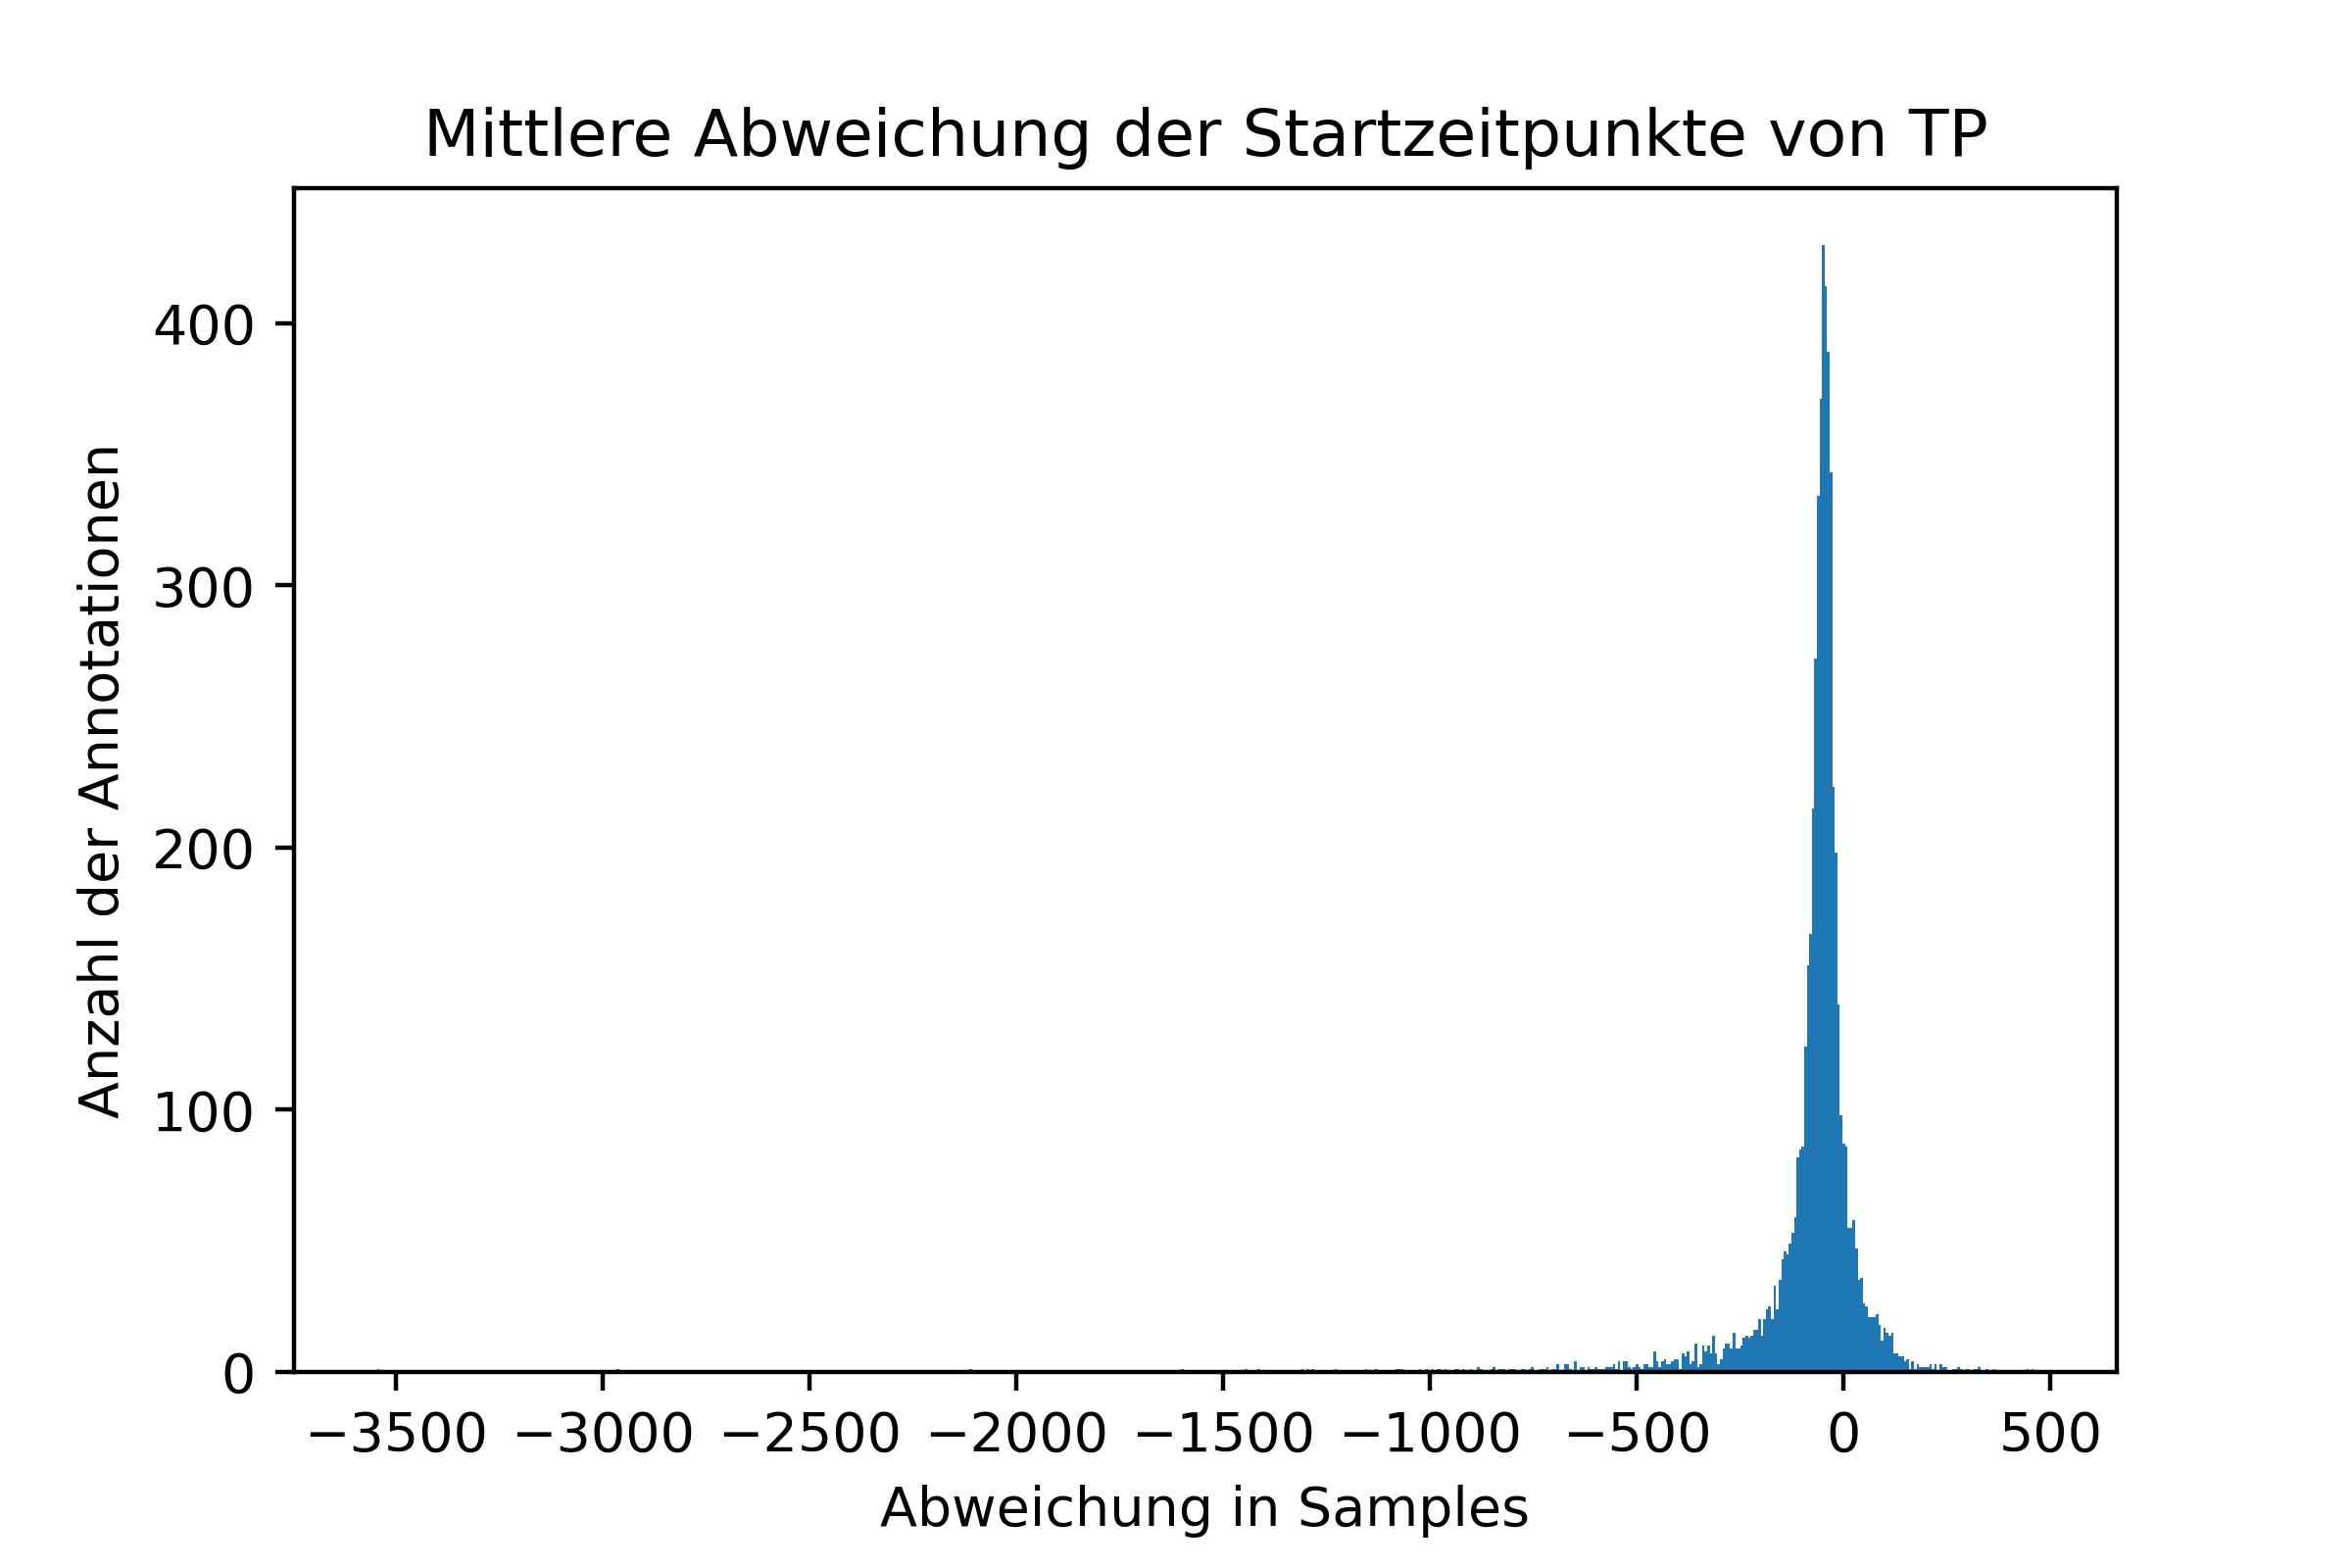
\includegraphics[width=0.80\textwidth]{./Bilder/LMStartDistribution_means.jpg}
	\end{center}
	\caption{Histogramm über die Mittlere Abweichung der Startzeitpunkte von TP bei einer Abtastfrequenz von 200 Hertz}%
	\label{fig:AASMKrit}%
\end{figure}

\begin{figure}[!ht]%
	\begin{center}
	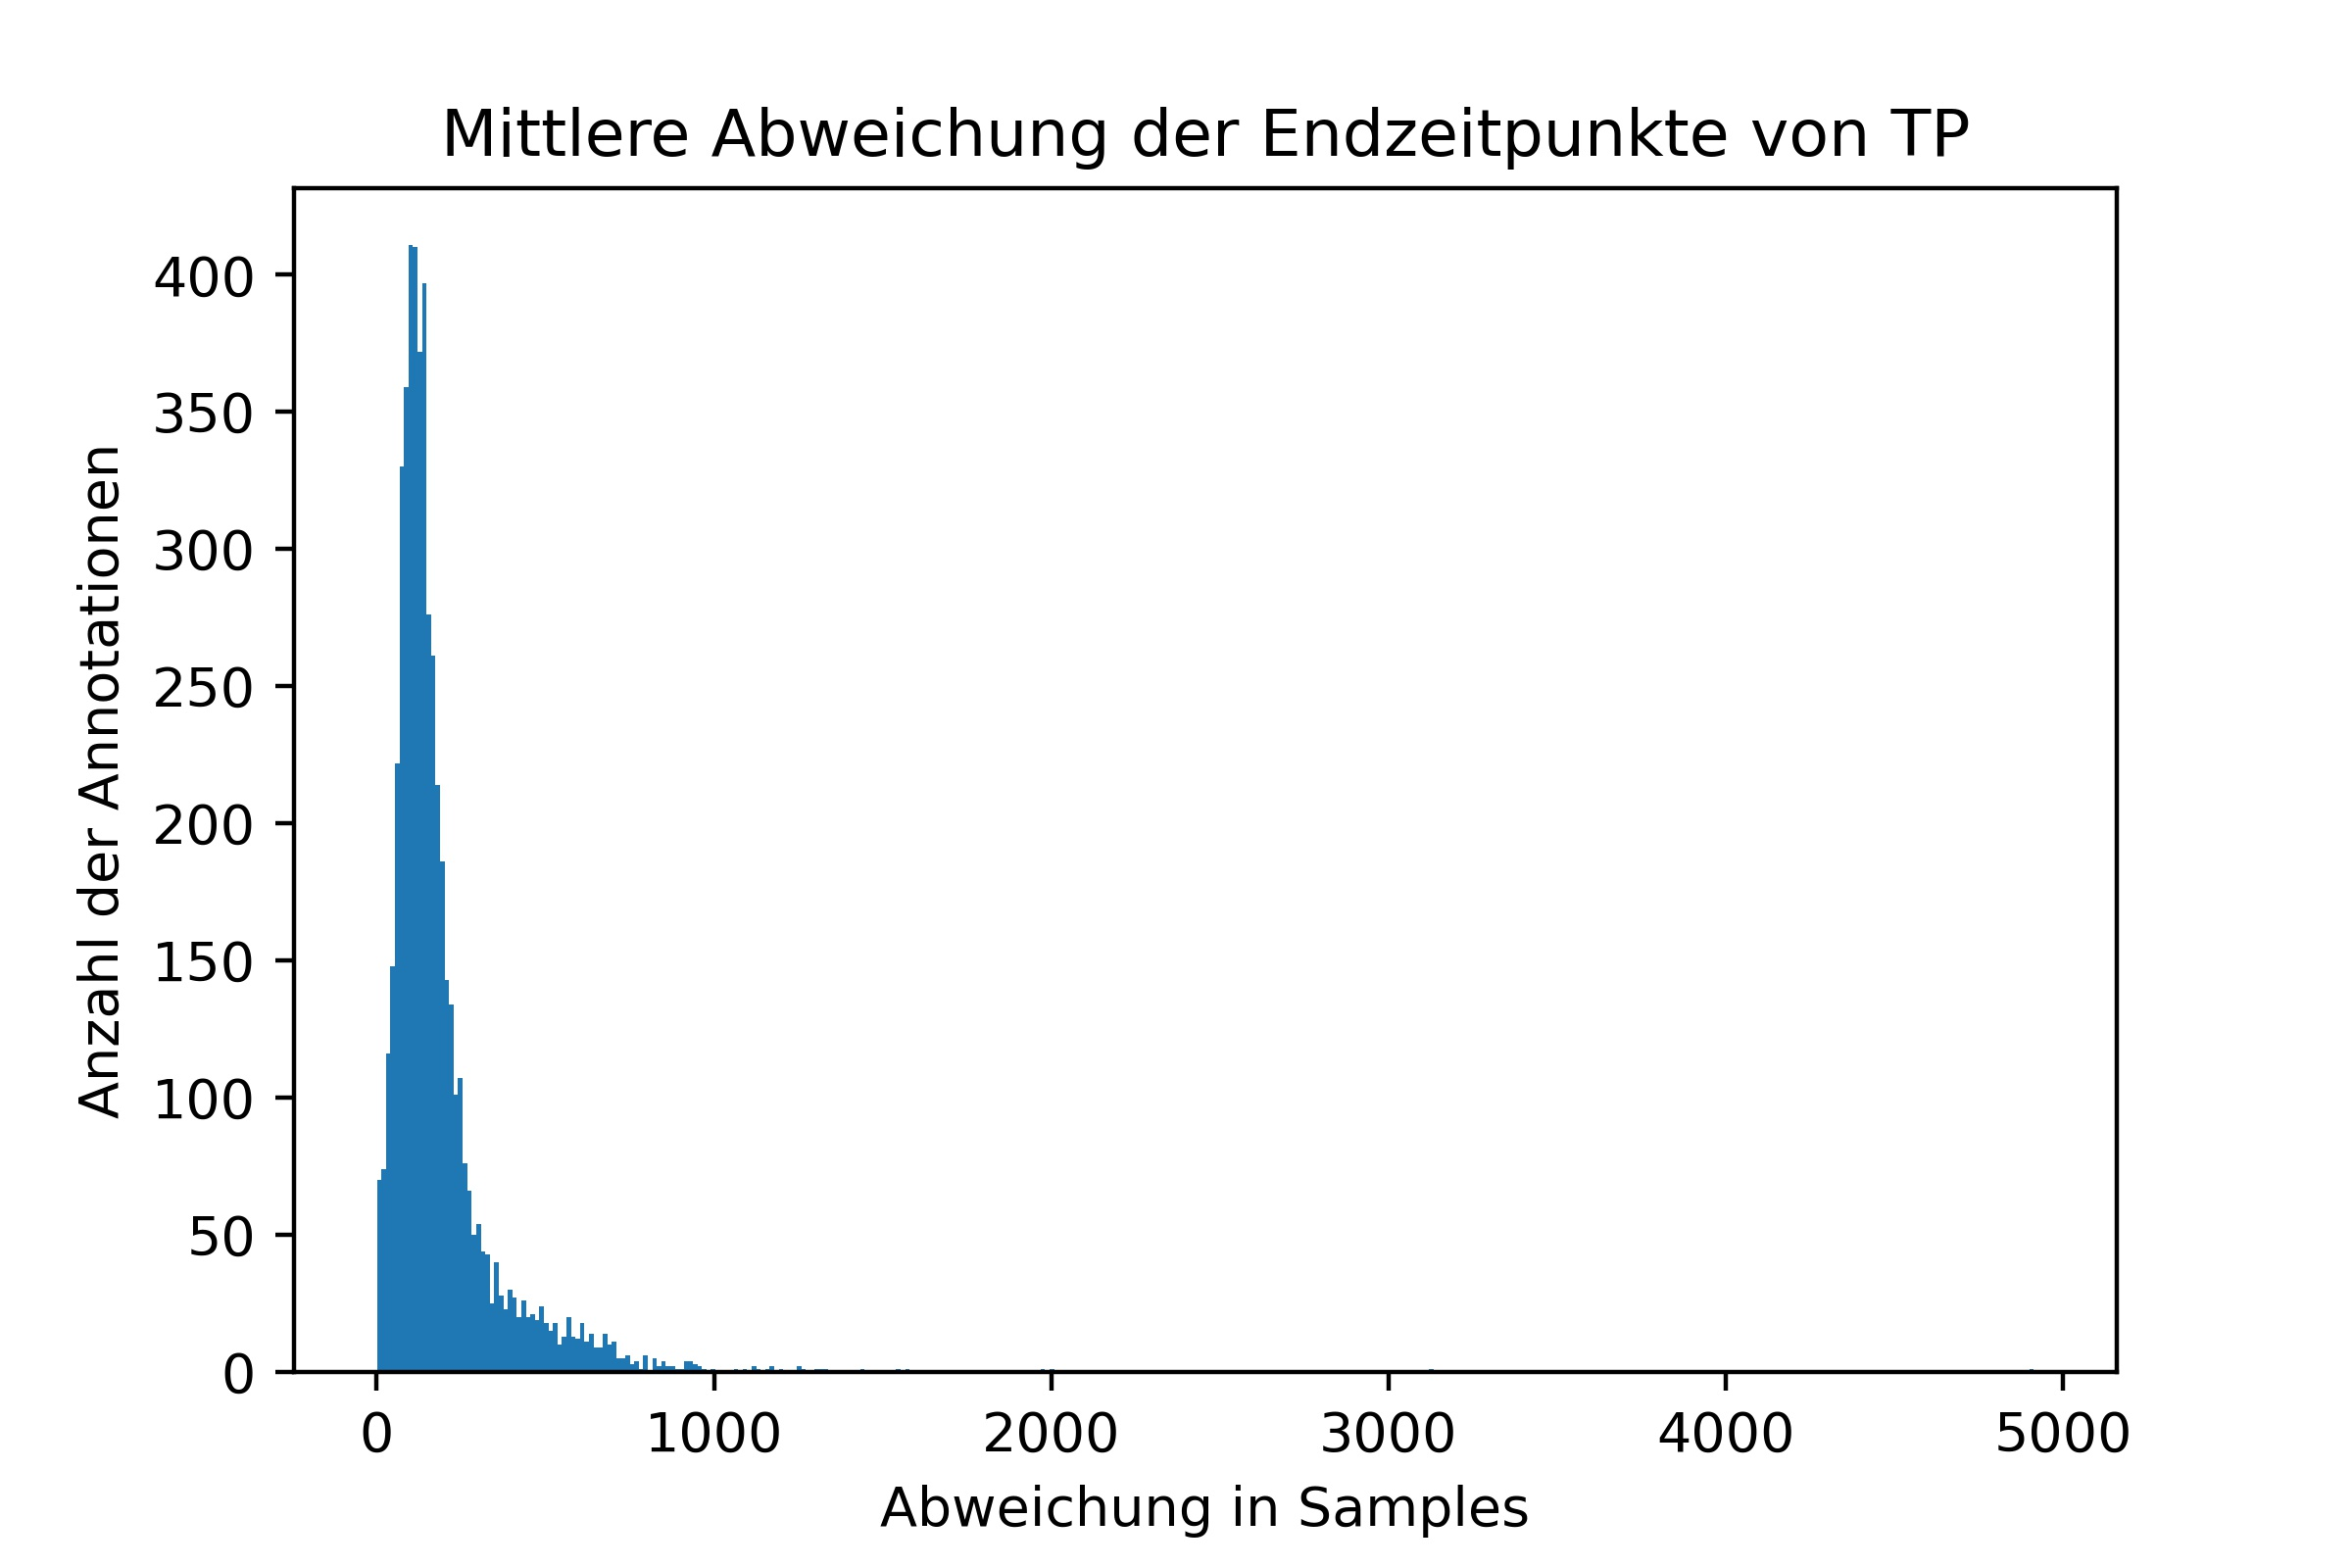
\includegraphics[width=0.80\textwidth]{./Bilder/LMEndDistribution_means.jpg}
	\end{center}
	\caption{Histogramm über die Mittlere Abweichung der Endzeitpunkte von TP bei einer Abtastfrequenz von 200 Hertz}%
	\label{fig:AASMKrit}%
\end{figure}


\begin{figure}[!ht]%
	\begin{center}
	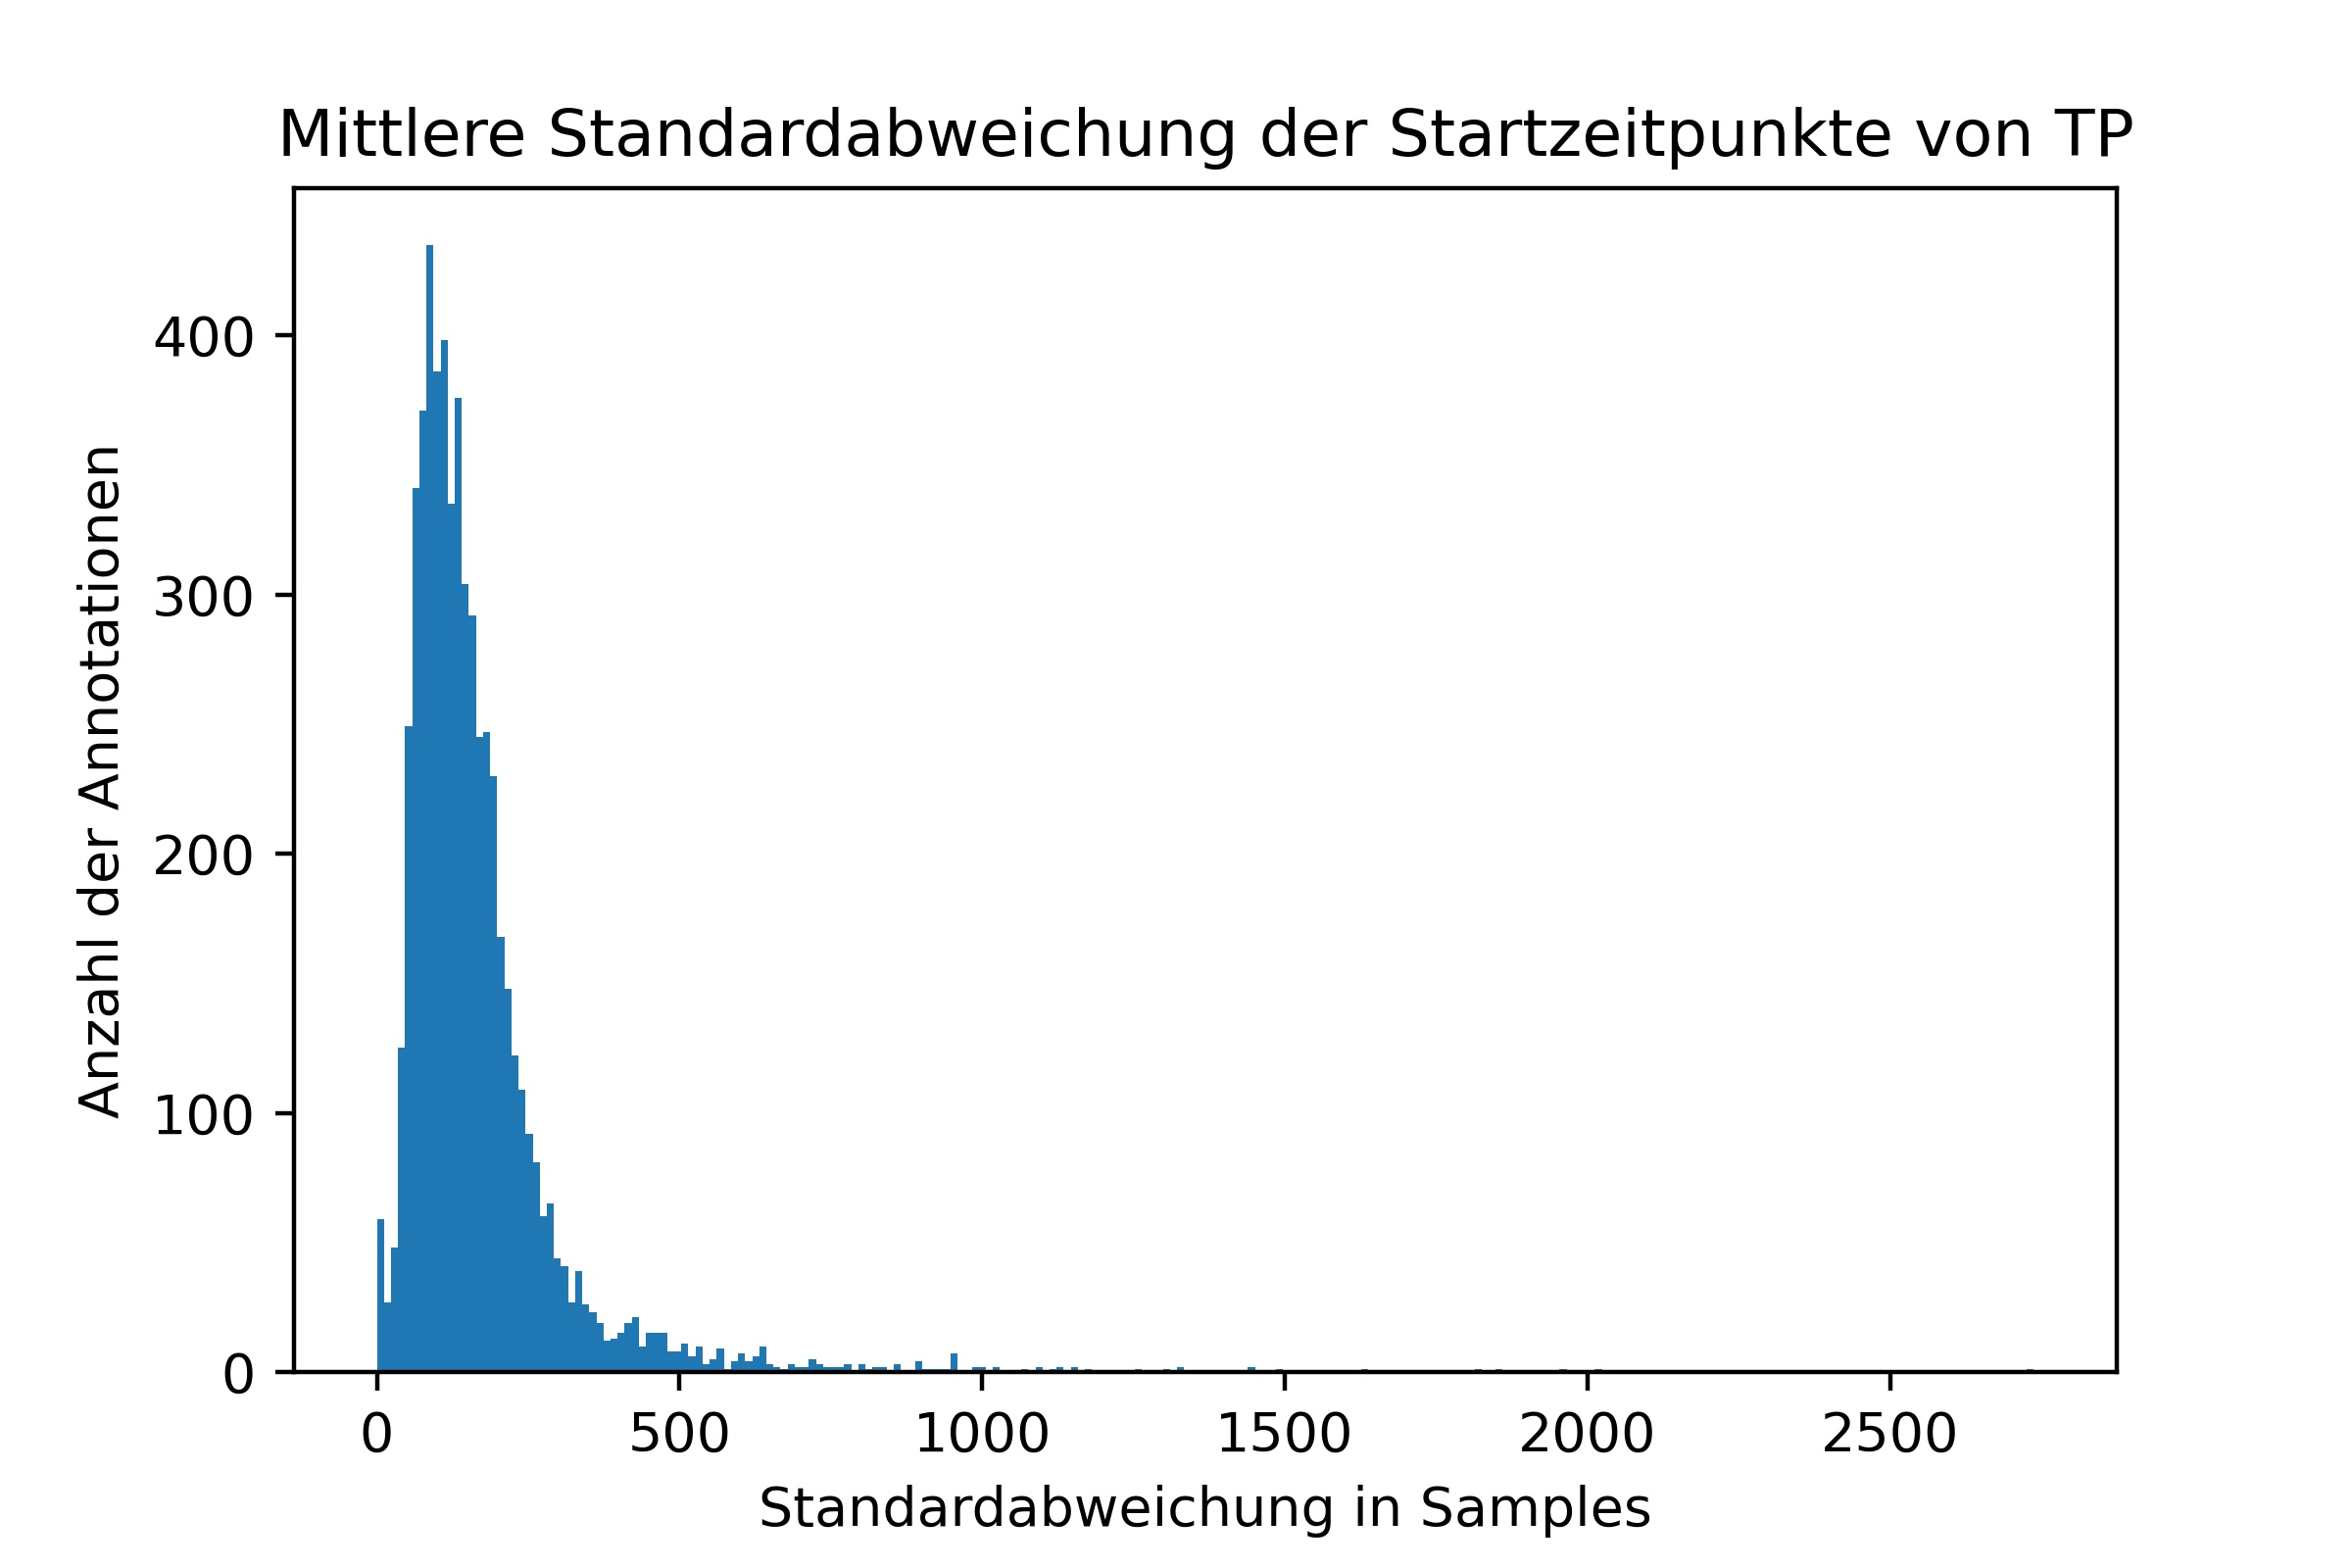
\includegraphics[width=0.80\textwidth]{./Bilder/LMStartDistribution_stds.jpg}
	\end{center}
	\caption{Histogramm über die Standardabweichung der Startzeitpunkte von TP bei einer Abtastfrequenz von 200 Hertz}%
	\label{fig:AASMKrit}%
\end{figure}

\begin{figure}[!ht]%
	\begin{center}
	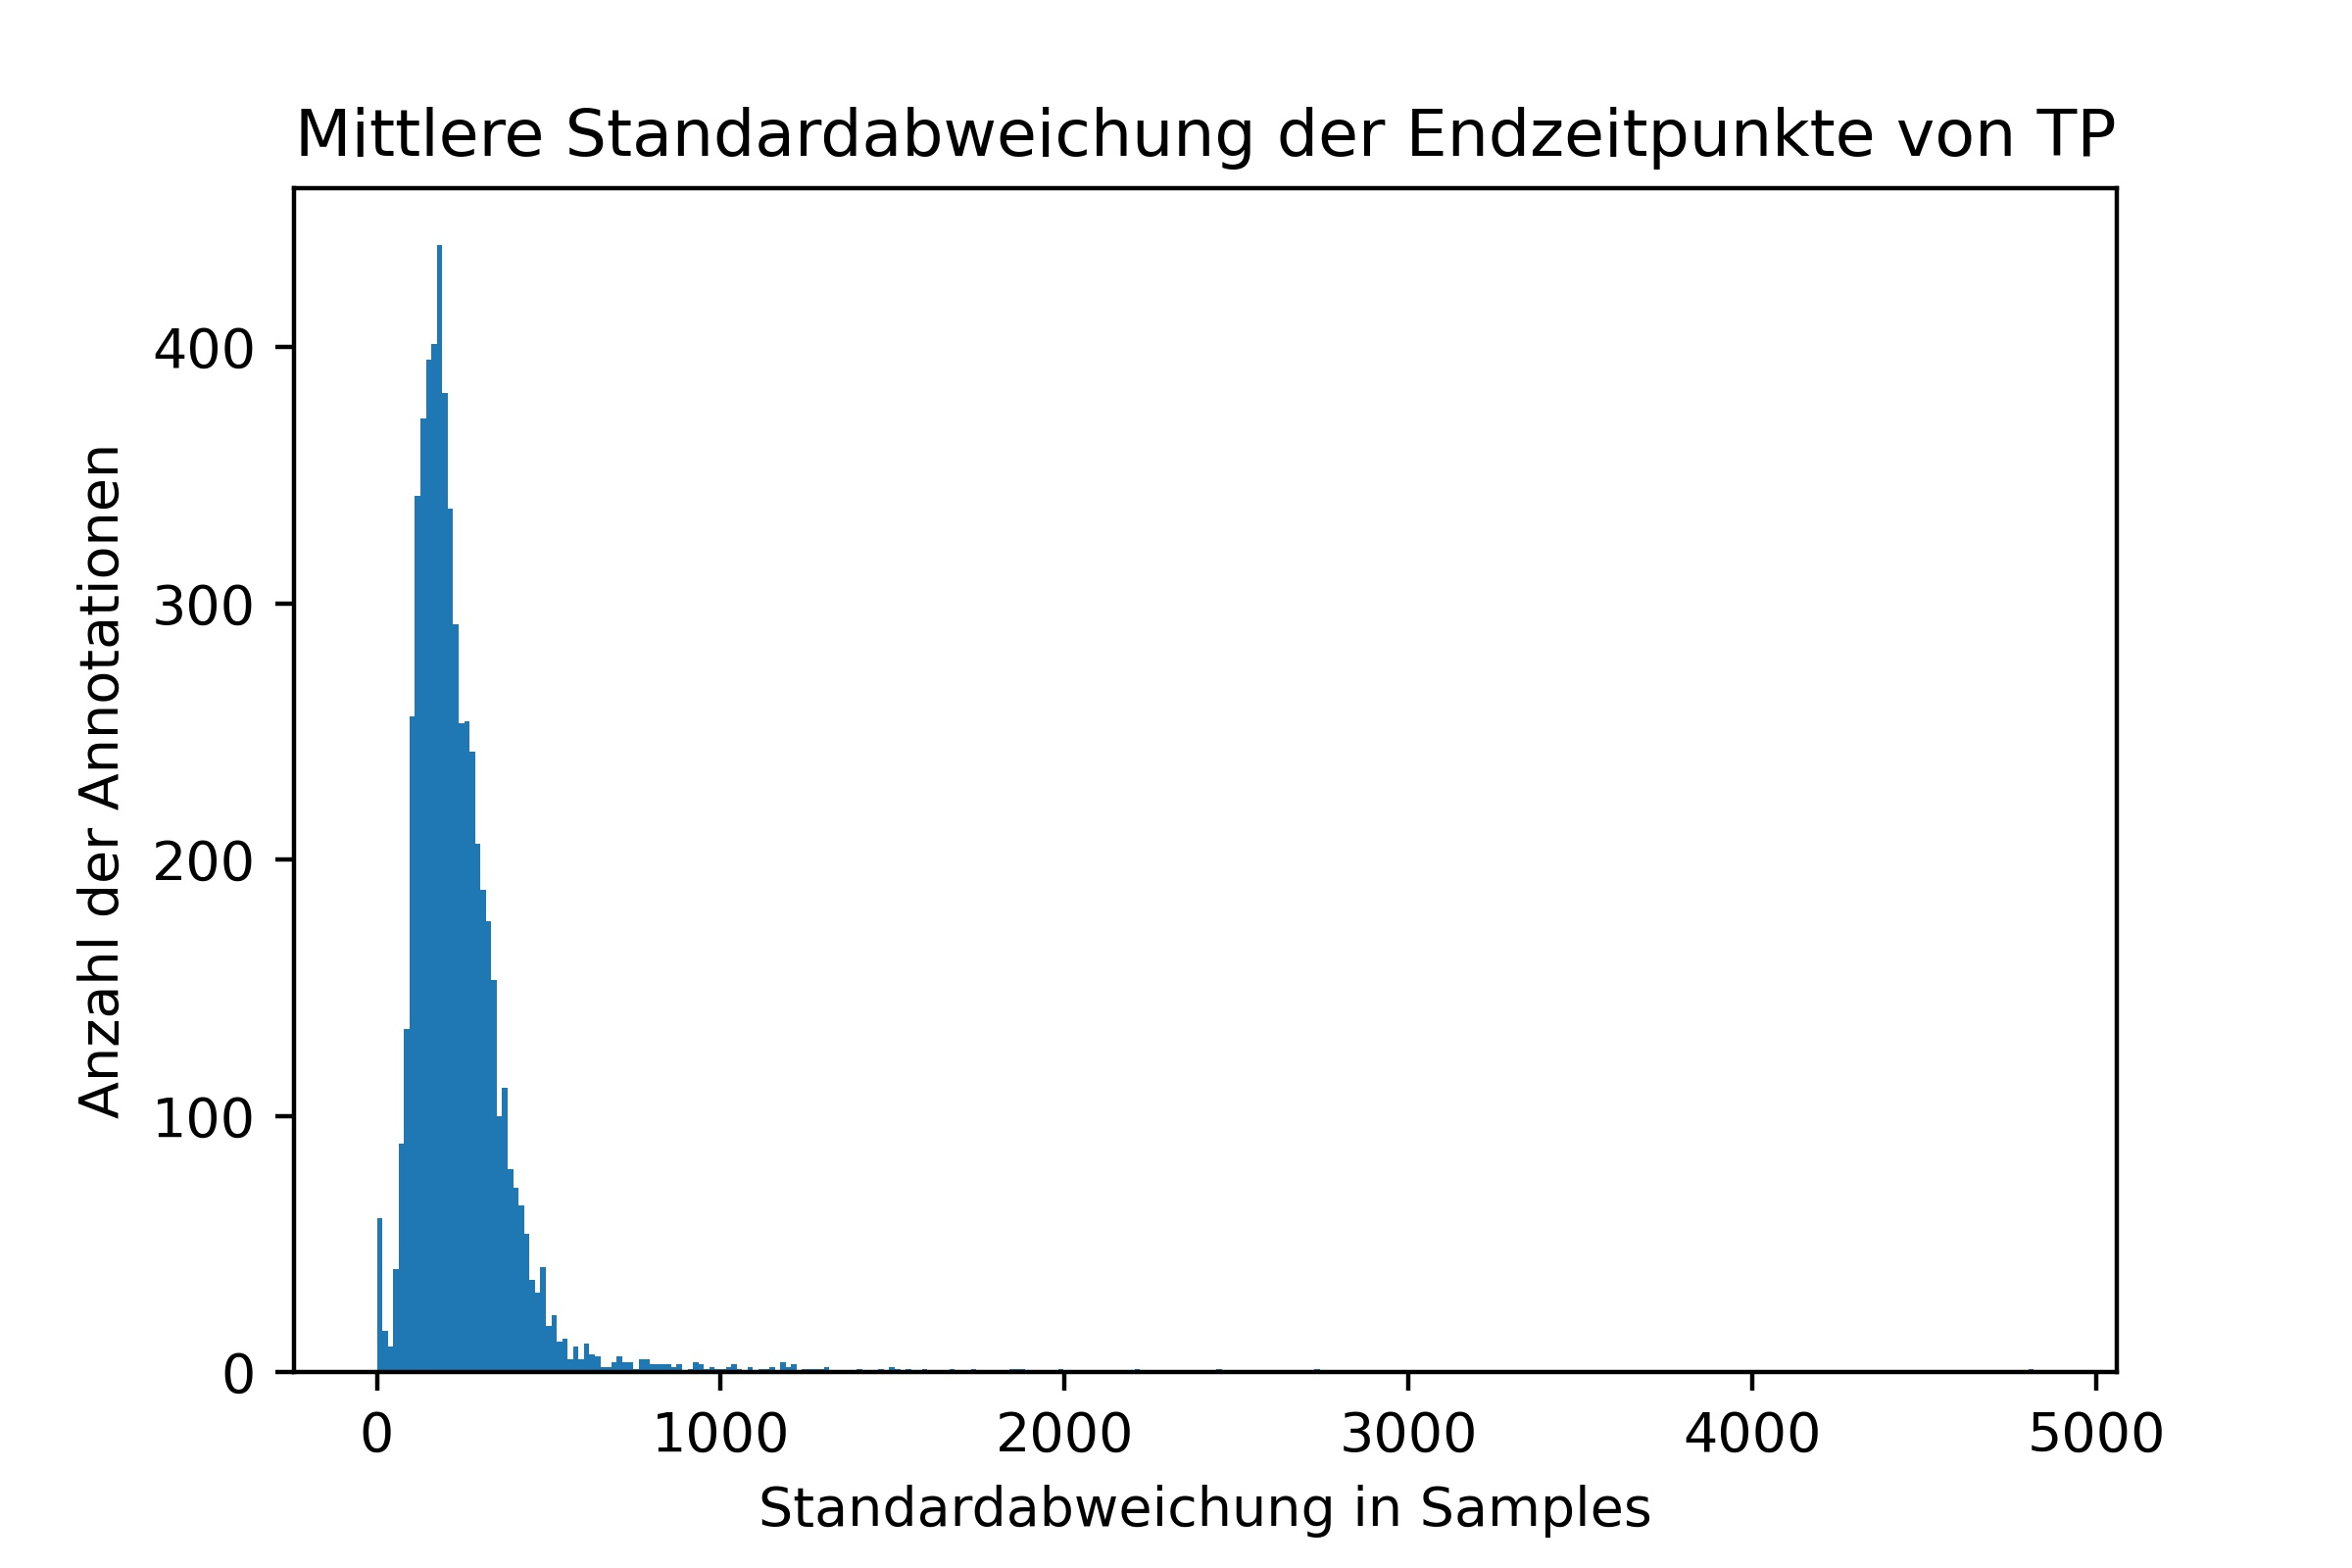
\includegraphics[width=0.80\textwidth]{./Bilder/LMEndDistribution_stds.jpg}
	\end{center}
	\caption{Histogramm über die Standardabweichung der Endzeitpunkte von TP bei einer Abtastfrequenz von 200 Hertz}%
	\label{fig:AASMKrit}%
\end{figure}

\begin{figure}[!ht]%
	\begin{center}
	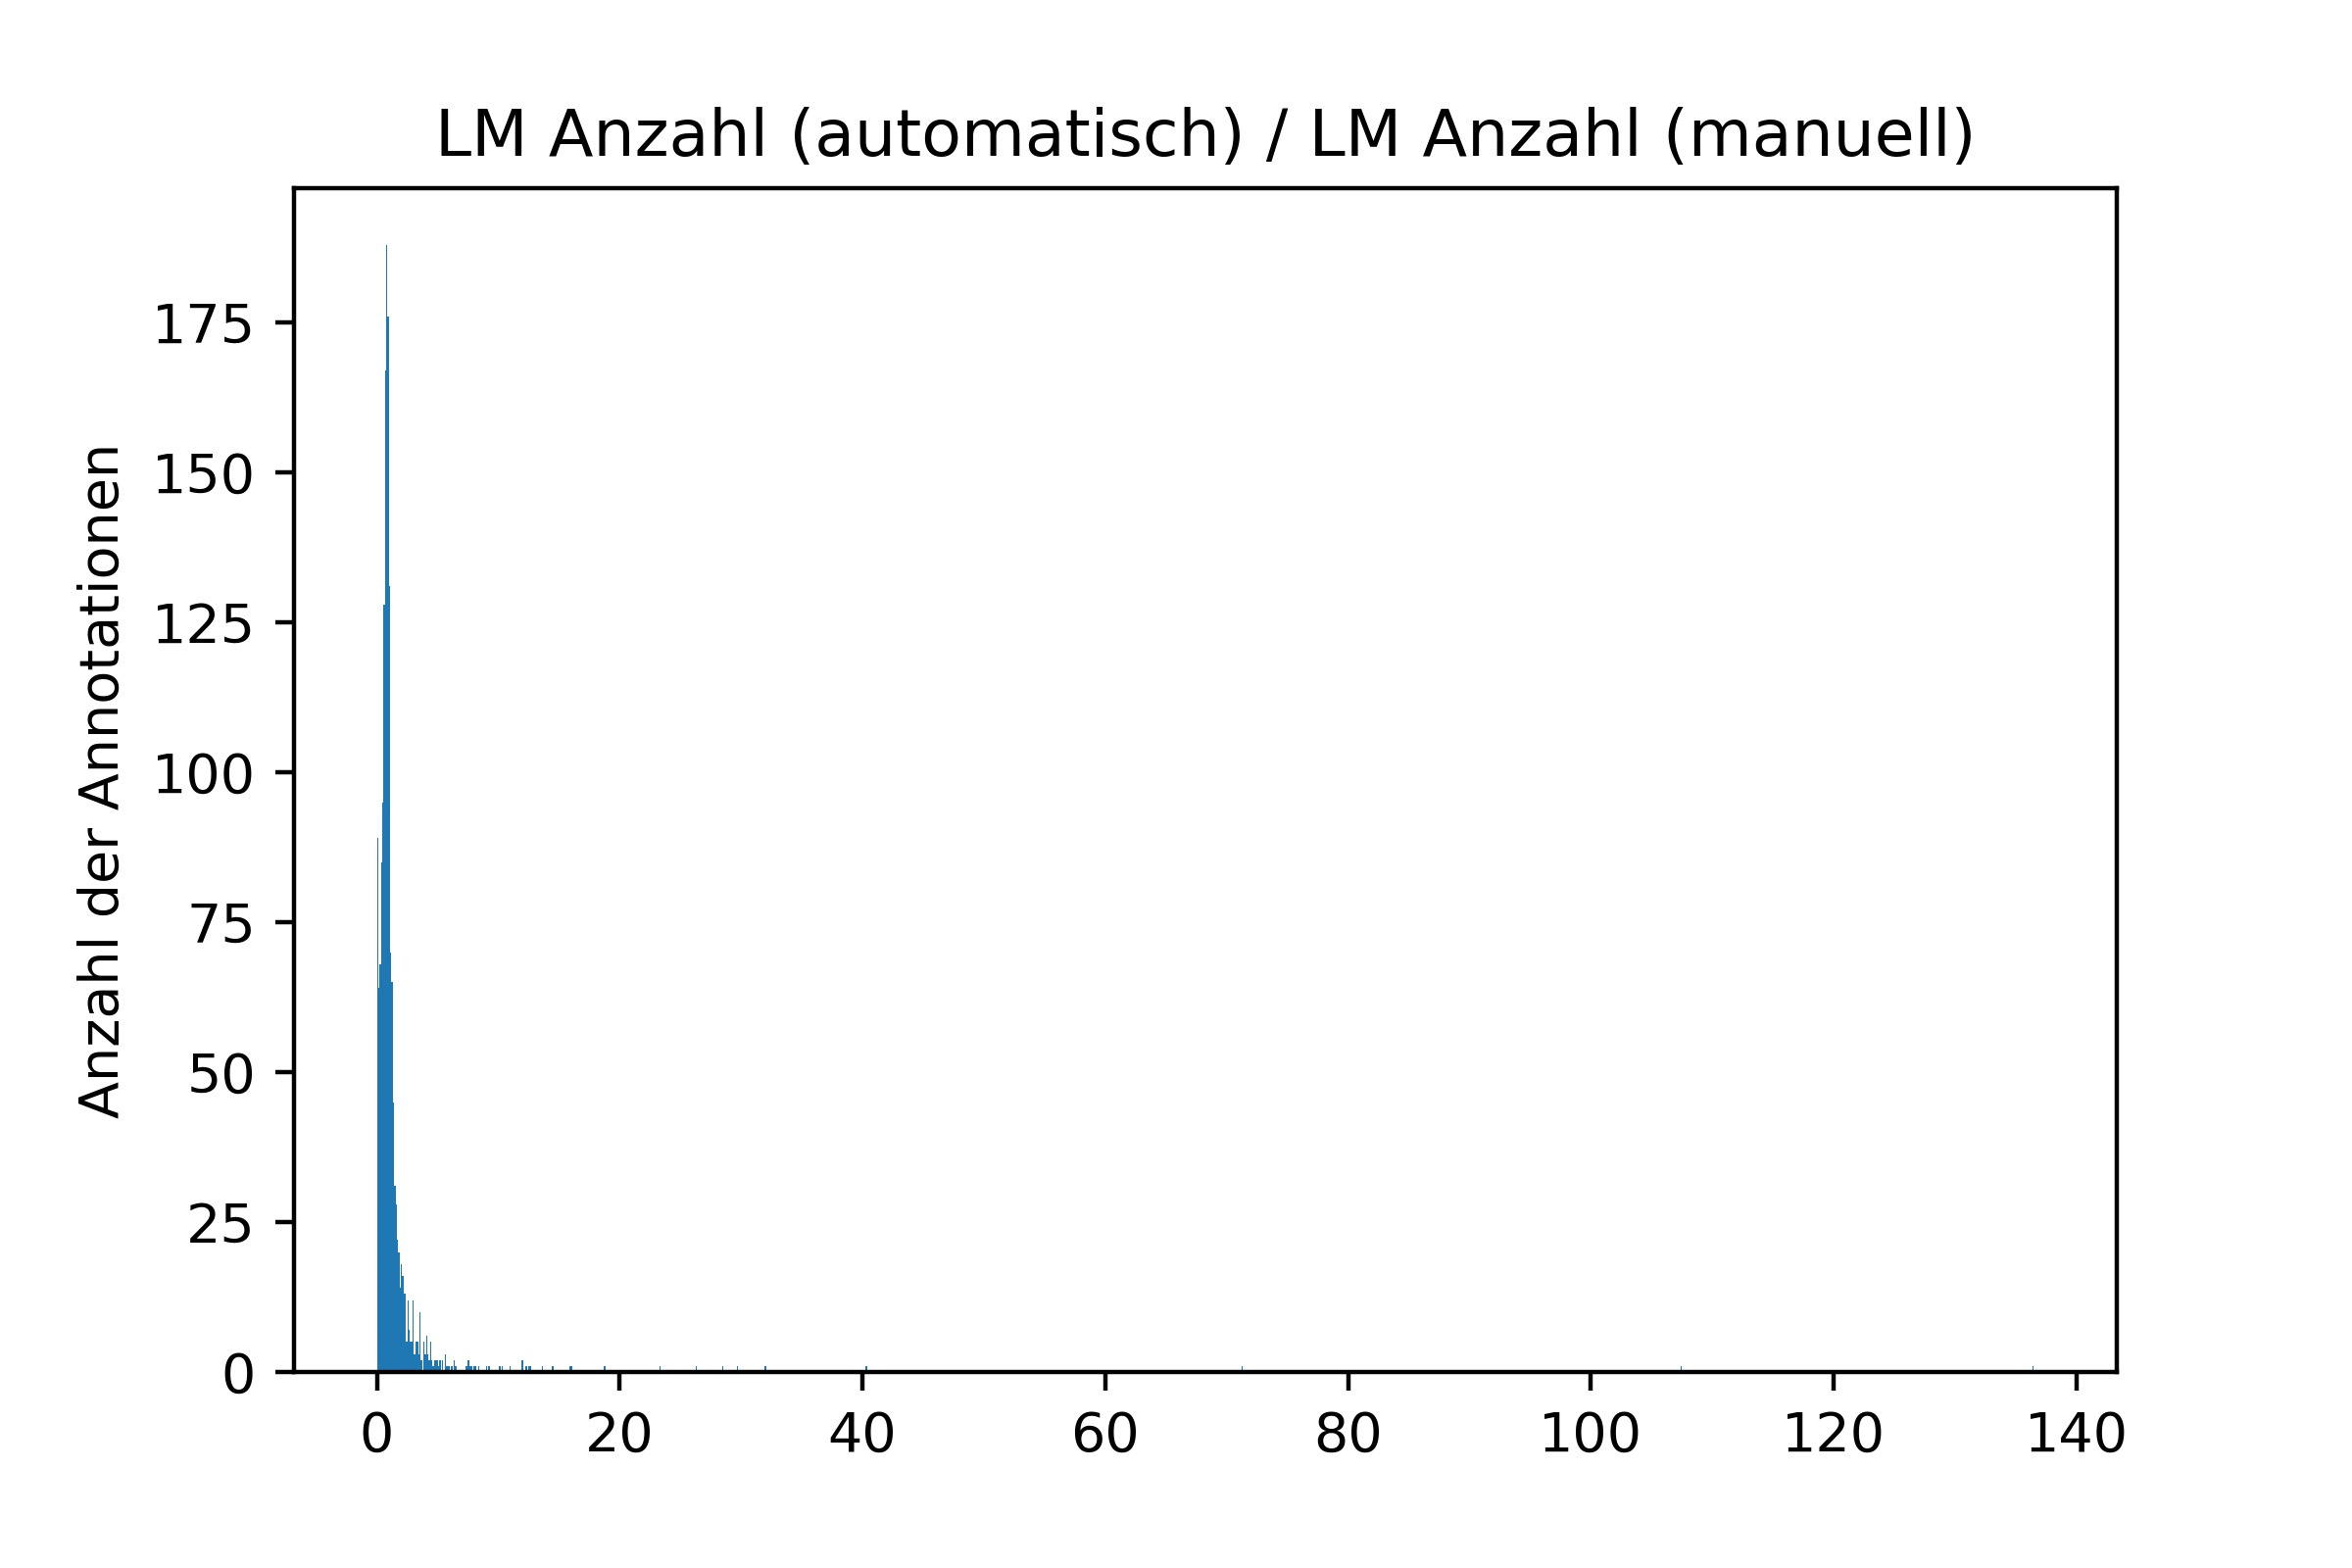
\includegraphics[width=0.80\textwidth]{./Bilder/LMcountrel.jpg}
	\end{center}
	\caption{Histogramm über das Verhältnis aus automatischer zu manueller LM Anzahl}%
	\label{fig:AASMKrit}%
\end{figure}


\begin{figure}[!ht]%
	\begin{center}
	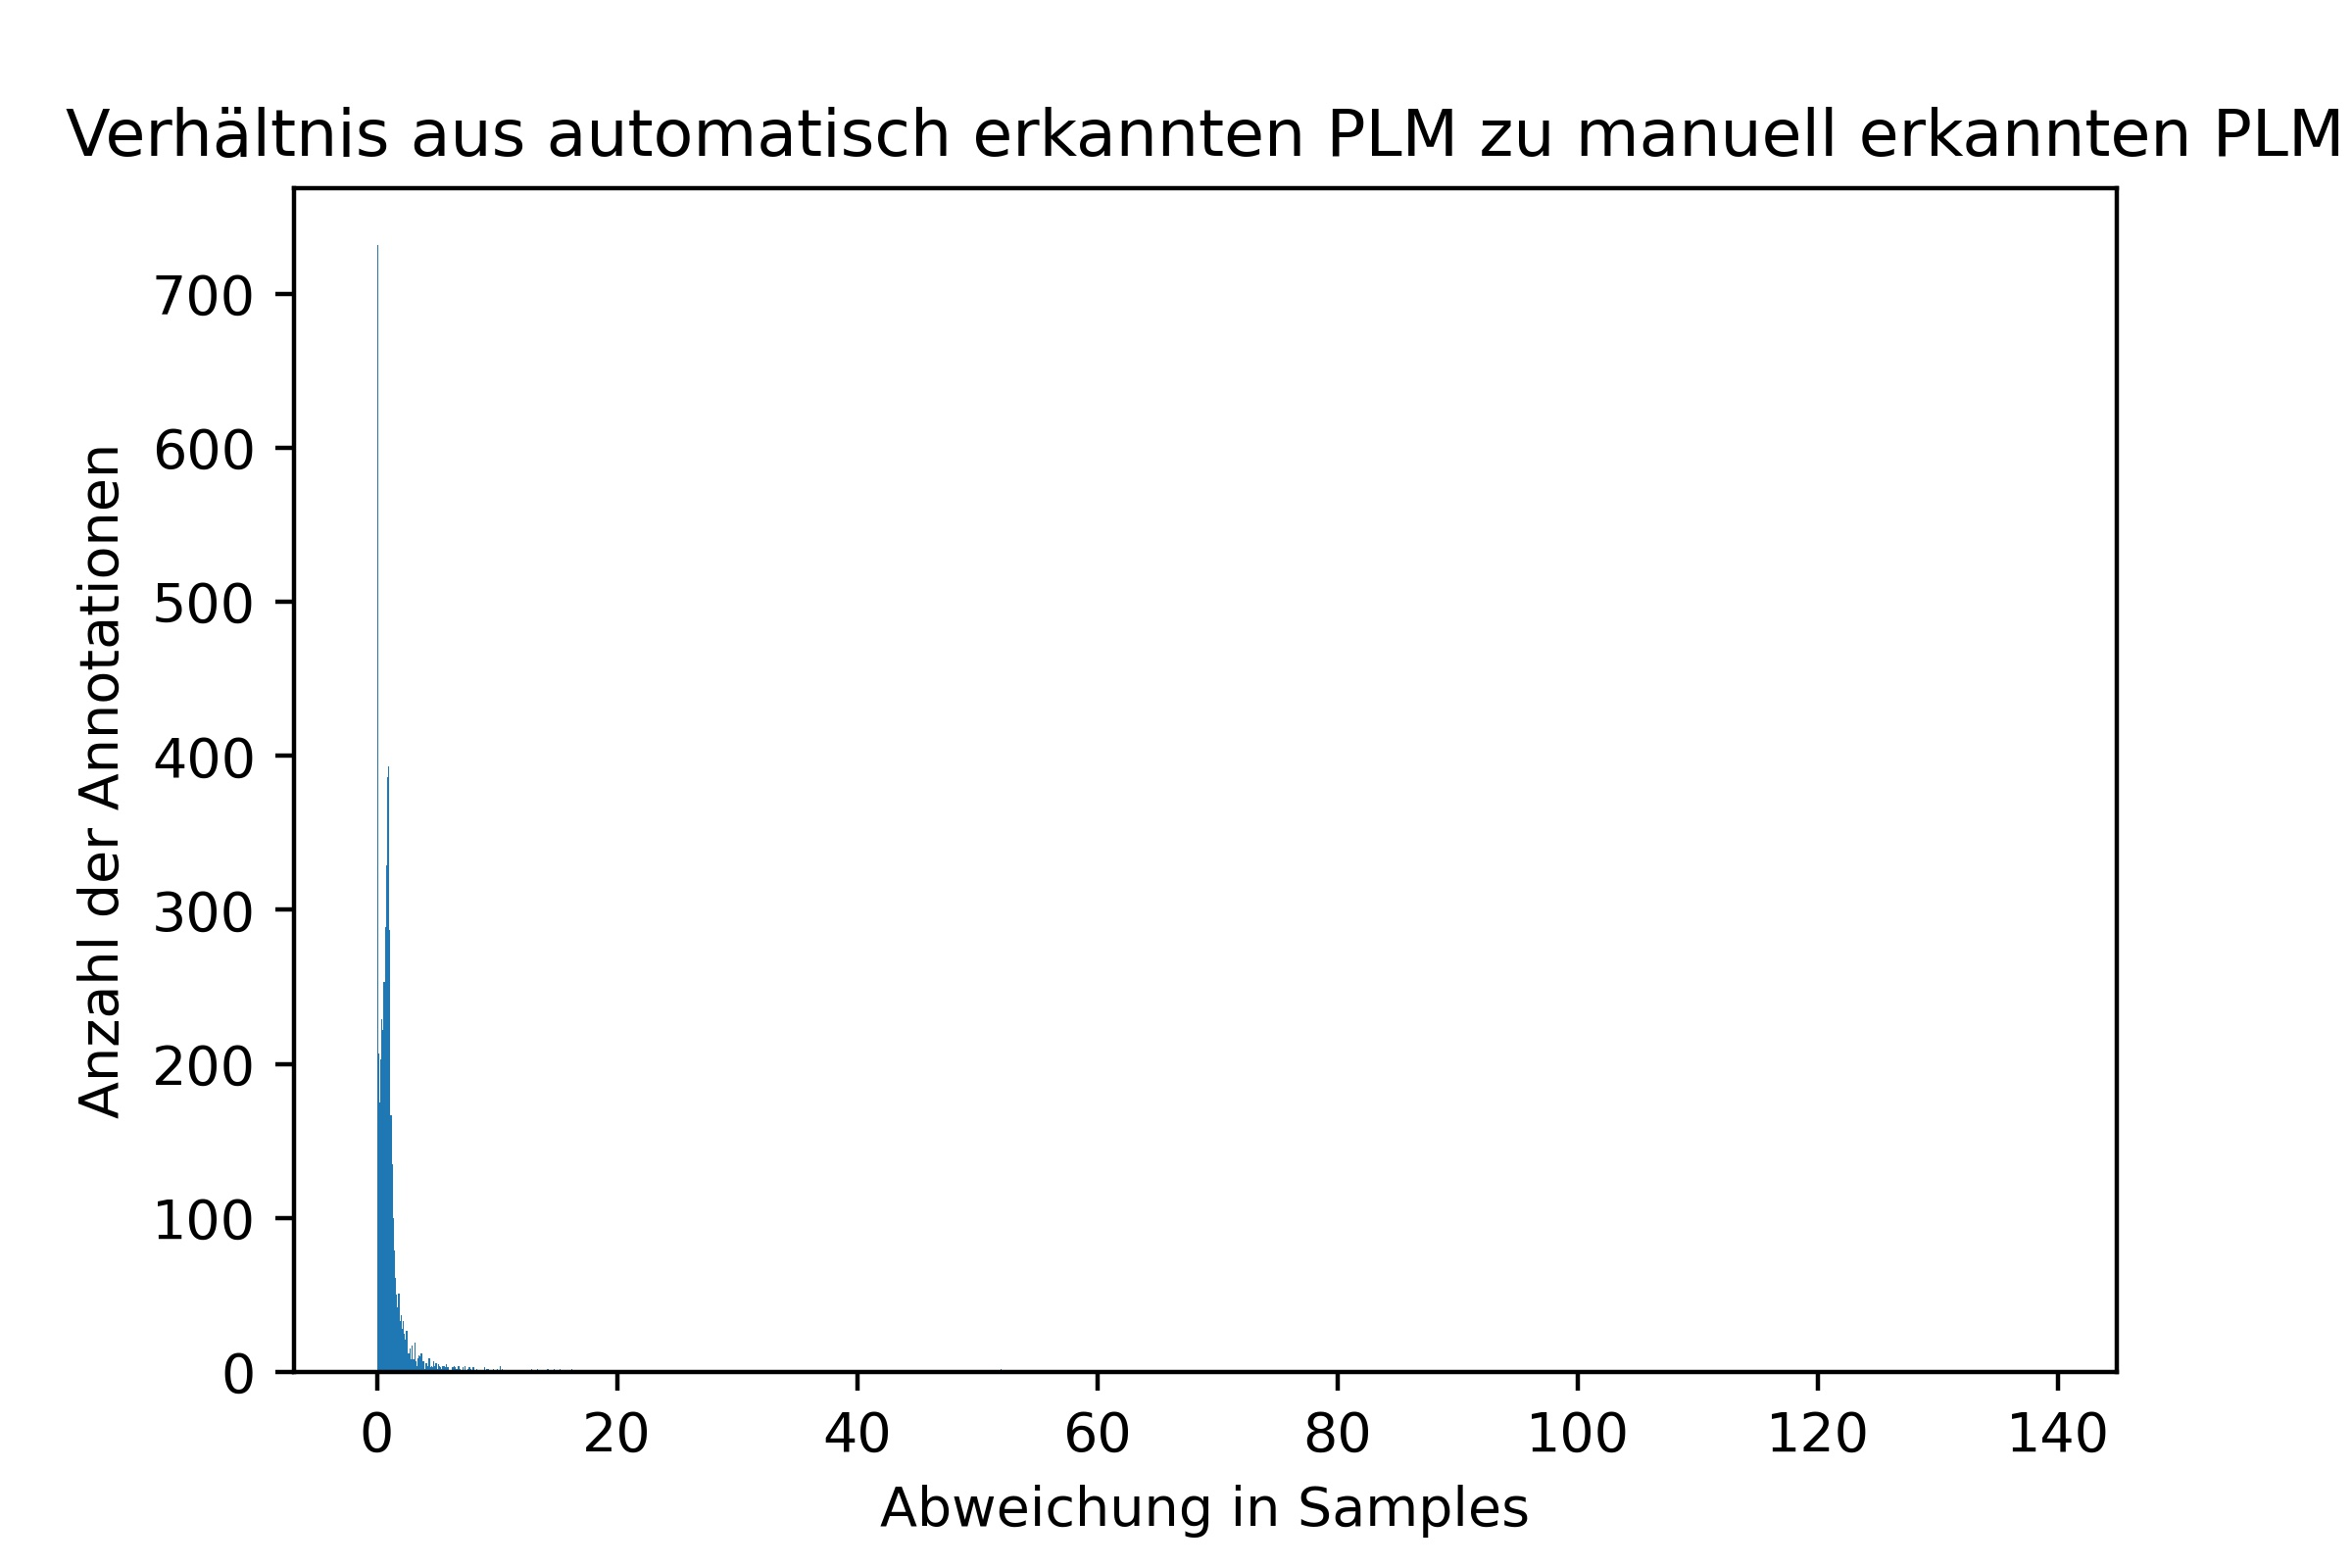
\includegraphics[width=0.80\textwidth]{./Bilder/Verhältnis aus automatisch erkannten PLM zu manuell erkannten PLM.jpg}
	\end{center}
	\caption{Histogramm über das Verhältnis aus automatischer zu manueller PLM Anzahl}%
	\label{fig:AASMKrit}%
\end{figure}

